\documentclass[12pt]{article}
\usepackage{pgf, tikz}
\usepackage{amsmath, amsfonts, amssymb, graphicx}
\usepackage{float}
\usepackage{subfig}
\usepackage[utf8]{inputenc}
\usepackage[spanish]{babel}
\usepackage{listings}
\usepackage{amsthm}
\usepackage{caption}

\setlength{\textheight}{23cm} \setlength{\evensidemargin}{0cm}
\setlength{\oddsidemargin}{-.5cm} \setlength{\topmargin}{-3cm}
\setlength{\textwidth}{17.5cm} \setlength{\parskip}{.2cm}


%opening

\begin{document}
	\begin{picture}(80, 80)
	\put(170,0){\hbox{
\includegraphics[scale=0.6]{cimat_logo.png}}}
	\end{picture}
	
	\begin{center}
		\begin{huge}
			Centro de Investigación en Matemáticas, A.C.
		\end{huge}
	\end{center}

	\begin{center}
		\begin{large}
			Descripción tarea 9 - Análisis de datos
		\end{large}
	\end{center}
	
	\begin{center}
		\textbf{Erick Salvador Alvarez Valencia}
	\end{center}

	\begin{center}
		15 de Noviembre de 2017
	\end{center}



%\maketitle

%\tableofcontent

\section{Descripción}
En el problema 2 de la tarea 9 se pide simular una distribución condicional que debemos encontrar, añadido a eso también se debe simular una distribución marginal de la variable $X$ para lo cual se calculan sus respectivas densidades y posteriormente las distribuciones acumulativas.\\
Para poder simular estas distribuciones partiendo de una uniforme debemos calcular las inversas de las ya mencionadas, quedando como resultado:

$$F_x^{-1}(x) = 2 \sqrt U_1$$
$$G_{Y|X=x}^{-1}(y) = \frac{U_2 X}{2}$$

Donde $U_1$ y $U_2$ son variables aleatorias con distribución uniforme. Para la simulación se creó un vector de 100 entradas y se hicieron 100 pruebas. Cada prueba consistía en calcular dos vectores de tamaño 100 que tuvieran valores de las distribuciones mencionadas anteriormente, para ello se tuvieron que calcular valores de la distribución uniforme y sustituirlos en las funciones anteriores. Al calcular dichos vectores se aplicó la función de covarianza en los mismos y el resultado se almacenó en el vector mencionado al comienzo.\\
Al concluir la simulación se verificó cómo se comportaban las covarianzas obtenidas y se determinó que su distribución se asemeja a la Normal con parámetros $\mu = 0.05$ y $\sigma^2$. A continuación se mostrará el código usado y posteriormente las gráficas de la densidad de la distribución de las covarianzas y un QQPlot que las compara con valores de una Normal.\\

\begin{lstlisting}[language=R]
#Aqui se guardaran las covarianzas de cada simulacion
C <- rep(100)
for(i in 1:100) {
	U1 <- runif(100, 0, 1)
	U2 <- runif(100, 0, 1)
	#Distribucion inversa a la marginal de X
	X <- 2 * sqrt(U1)
	#Distribucion inversa a la condicional de Y dado X
	Y <- (U2 * X) / 2
	C[i] <- cov(X, Y)
}

#Se proyecta la densidad de las covarianzas
plot(density(C))

#Hacer un QQPlot
qm <- sort(C)
qt <- rnorm(100)
qqplot(qt, qm, xlab="Cuantil teorico", ylab="Cuantil muestral")
qqline(qm, col = 2)
\end{lstlisting}

A continuación se muestran las gráficas obtenidas:
\begin{figure}[H]
	\centering
	\subfloat[][Figura 1. Densidad generada del vector de covarianzas.]{
		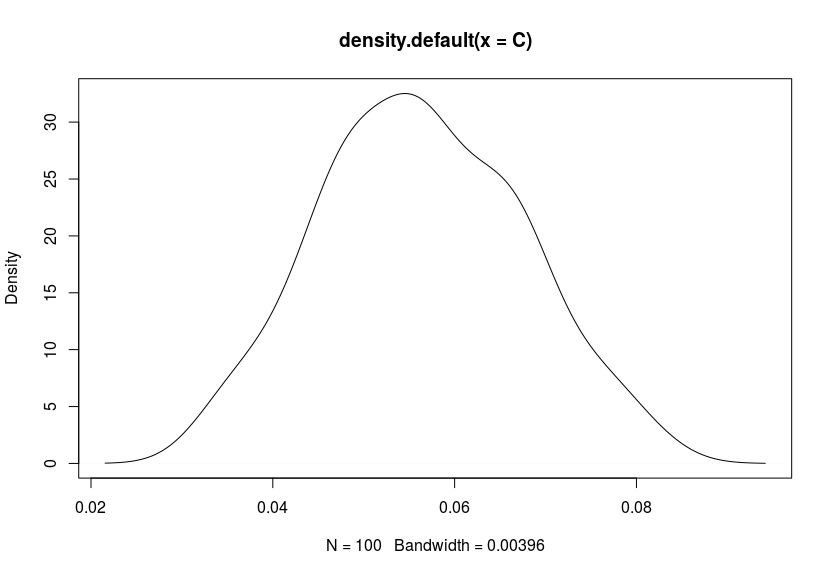
\includegraphics[scale=0.5]{N1.png}
	}\hfill
\end{figure}

\begin{figure}[H]
	\centering
	\subfloat[][Figura 2. QQPlot del vector de covarianzas comparado con datos de una distribución normal.]{
		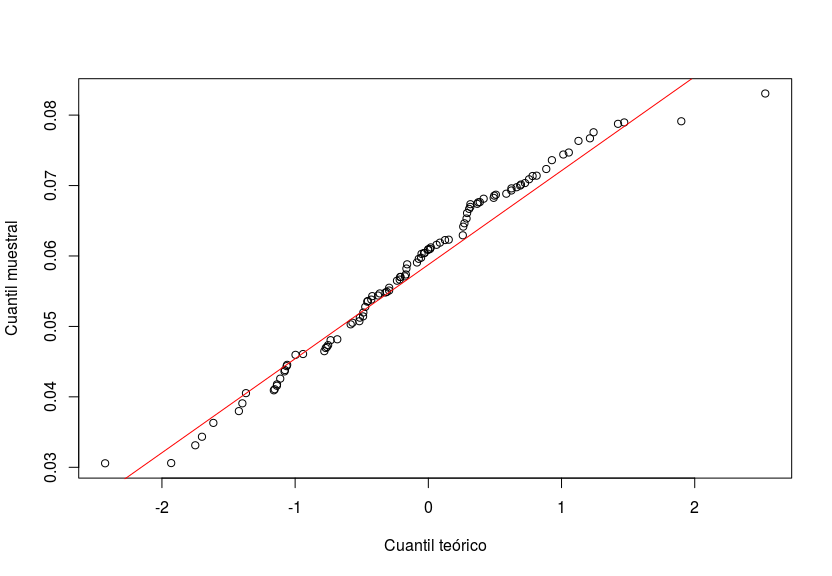
\includegraphics[scale=0.5]{QQ1.png}
	}\hfill
\end{figure}

Podemos ver en la Figura 1. la similitud de la densidad comparada con la de una normal centrada en $0.05$ lo que se obtuvo en el cálculo que se pide en el ejercicio $\frac{1}{18}$, y de la misma forma en la Figura 2. el QQPlot de las distribuciones está casi centrado en la recta identidad lo cual indica un alto grado de similitud.

\end{document}
